\documentclass[11pt]{article}
\usepackage{ctex}
\usepackage{graphicx}
\usepackage{amssymb}
\usepackage{amsmath}
\usepackage{algorithm}
\usepackage{algorithmic}
\usepackage{hyperref}
\usepackage{geometry}
\usepackage{fancyhdr}
\geometry{left=3.0cm,right=3.0cm,top=3.0cm,bottom=3.0cm}
\pagestyle{fancy} 

\begin{document}
\begin{titlepage}
    \begin{center}
    \phantom{Start!}
    \vspace{3cm}
       \center{\zihao{2}\kaishu 统计信号处理第二次大作业}
        {
        \setlength{\baselineskip}{40pt}
        \vspace{1cm}
        \zihao{-1}
        \center{\kaishu ~~最小二乘法应用~~}
        \vspace{3.5cm}
        \zihao{-3}
        \center{
          \begin{tabular}{cccc}
          姓名: & 刘\quad 前 \\
          学号:& 2014011216 \\
          班级:& 无47\\
          日期:& 2017-06-24\\
          \end{tabular}
        }
        \vspace{4cm}
        }
    \end{center}
\end{titlepage}


\begin{center}
\tableofcontents
\end{center}

\newpage
\twocolumn
\begin{abstract}
{\kaishu
协同滤波是推荐系统中常用的推荐算法之一。本次大作业基于协同滤波这一问题背景,尝试使用加权正则化交替最小二乘法解决了协同滤波中的填充矩阵问题,其基本思想是使用交替最小二乘法优化二次误差函数。除此之外,本文还实现了正则奇异值分解的方法,但是未利用最小二乘的思想,因而不在报告中详细介绍。加权正则化交替最小二乘法是本次大作业重点呈现的算法,有效解决了协同滤波问题。本文着重对该算法超参数的选择、性能评价(测试集上的均方误差)和算法的收敛速度进行了分析与讨论,最终得到了性能较优的结果。
}
\end{abstract}

\section{问题背景}
推荐系统是目前非常活跃的研究方向之一,主要目的是利用用户的评分记录等信息对用户进行推荐。推荐系统包含了很多推荐算法,其中最常用的算法是协同滤波。

协同滤波经典背景是:假设有$n_u$个用户和$n_i$部电影(也可以是商品、美食等其他物品),用户u对电影i的打分记作$M_{ij}$,由此可以形成一个大小为$n_u\times n_i$的评分矩阵M。实际生活中每个用户不一定对所有的电影都打过分,所以矩阵M不会被完全填充,因而协同滤波所要解决的问题也可以归纳为填充矩阵问题,即:根据现有的打分信息,估计得到整个评分矩阵M\cite{Net}。


\section{最小二乘法简介}
最小二乘法应用十分广泛,尤其在函数逼近、数据拟合和回归分析等领域,是最重要的方法之一。首先,从狭义上理解,最小二乘法主要可以概括为:给定二次误差函数$L(\textbf{y},\hat{\textbf{y}}) = \vert\vert \textbf{y} - \hat{\textbf{y}} \vert\vert_{2}^{2}$下,利用该在样本点上预测值与样本值间的误差总和$L = \sum_{i=1}^{N}L(\textbf{y}_{i},\hat{\textbf{y}(\textbf{x}_{i})})$最小确定数学模型$\hat{\textbf{y}}(x)$。

需要注意的是,最小二乘法的使用前提是:给定数学模型$\hat{\textbf{y}}(x)$的函数形式$f(\textbf{x},\theta)$,当此函数相对于模型参数$\theta$是非线性函数时,此问题即为非线性最小二乘问题,否则即为有闭式解的线性最小二乘问题。

近年来,最小二乘问题又有很多扩充内容,一类是针对模型参数$\theta$进行约束或者限制,比如:等式约束、稀疏性约束、能量最小化约束等等。也有对拟合模型$\hat{\textbf{y}}(x)$进行约束的,比如光滑性约束等,这类问题可以转化为普通最小二乘问题,或者利用迭代重加权最小二乘方法求解。另一类是优化参数具有多重线性性,可以使用交替最小二乘方法求解。

\section{加权正则化交替最小二乘法}
\subsection{算法目标}
加权正则化交替最小二乘法(Alternating-Least-Squares with Weighted-λ Regularization,后文简称为ALS-WR)是最小二乘法的一种变体。对于填充矩阵问题,ALS-WR算法的思路和目标如下。

将所要填充的矩阵表示为:$\textbf{M} = \textbf{U}\textbf{V}^{\rm T}$,其中$M_{ij} = \textbf{U}(i,:)\textbf{V}(j,:)^{\rm T}$,表示用户i对电影j的打分是用户i的隐变量$\textbf{U}(i,:)$与电影j的隐变量$\textbf{V}(j,:)$的内积。考虑到用户类型和电影类型有限,因而可以认为评分矩阵$\textbf{M}$是低秩的。由于矩阵的秩是矩阵奇异值向量的0范数,可以将其放缩到1范数(矩阵的核范数)。矩阵的核范数满足:
\begin{equation}
	\vert\vert\textbf{X} \vert\vert_{*} = \underset{\textbf{U},\textbf{V}\vert\textbf{X} = \textbf{U} \textbf{V}^{\rm T}}{\rm min} \frac{1}{2}(\vert\vert\textbf{U} \vert\vert_{F}^2 + \vert\vert\textbf{V} \vert\vert_{F}^{2})
	\label{X}
\end{equation}

因而,上述问题可以转换为求解优化下面的目标函数:
\begin{equation}
	\underset{\textbf{U}, \textbf{V}} {\rm min} = \vert\vert \textbf{W} * (\textbf{M} - \textbf{U}\textbf{V}^{\rm T}) \vert\vert_{F}^{2} + \frac{\lambda}{2}(\vert\vert \textbf{U} \vert\vert_{F}^{2} + \vert\vert \textbf{V} \vert\vert_{F}^{2})
	\label{loss}
\end{equation}

其中,需要说明的是:$\lambda$是控制矩阵低秩程度的超参数;\textbf{W}是标志矩阵,$W(i,j) = 1$表示用户i对电影j已经打过分,$W(i,j) = 0$表示未打分,*表示矩阵对应元素相乘。本次大作业ALS-WR算法针对于目标函数进行优化求解。

\subsection{算法原理}
目标函数(式\ref{loss})的优化问题可以使用交替最小二乘法进行求解。其核心思路是先固定其中一个变量,另一个变量作为优化变量使用最小二乘方法求解。比如,先固定\textbf{V},以\textbf{U}作为优化变量,使用最小二乘法进行更新;然后再固定\textbf{U},以\textbf{V}作为优化变量,如此交替,直至一定次数或者判断收敛\cite{ALSWR}。

根据算法目标,希望找到一个低秩矩阵\textbf{X}来逼近矩阵\textbf{M},其中$\textbf{M} = \textbf{U}\textbf{V}^{\rm T}$。设矩阵$\textbf{U}$为$m\times d$的矩阵,$\textbf{V}$为$n \times d$的矩阵。其中d表示特征的个数,若矩阵$\textbf{M}$的秩为r,则一般有$d << r$。为方便后文推导,不妨记$\textbf{U} = [u_1,u_2,\cdots,u_m]^{\rm T}$,$\textbf{V} = [v_1,v_2,\cdots,v_n]^{\rm T}$。

根据标志矩阵$\textbf{W}$的作用,不妨设矩阵$\textbf{M}$中的所有非零元素构成集合$\Omega$,则公式\ref{loss}可以转换为
\begin{equation}
	L = \sum_{i,j,(i,j)\in \Omega} (M_{ij} - u_{i}^{\rm T}v_{j})^2 + \frac{\lambda}{2}(\vert\vert u_{i} \vert\vert^2 + \vert\vert v_{j} \vert\vert^2)
	\label{loss2}
\end{equation}

下面使用交替最小二乘法使得损失函数(式\ref{loss2})最小。先固定\textbf{V},以U作为优化变量。将损失函数(式\ref{loss2})对$u_{i}$进行求导,则
\begin{equation}
	\frac{\partial L}{\partial u_{i}} = \sum_{j,(i,j)\in\Omega} 2(M_{ij} - u_{i}^{\rm T}v_{j})(- v_j) + 2\times\frac{\lambda}{2}u_i  = 0
	\label{ded}
\end{equation}
\begin{equation}
	\sum_{j,(i,j)\in\Omega} M_{ij}v_j = \frac{\lambda}{2}u_i + \sum_{j,(i,j)\in\Omega} u_{i}^{T}v_{j}v_{j}
	\label{sim}
\end{equation}

将公式\ref{sim}中的求和改写成向量的形式,则得到
\begin{equation}
	V_{i*}^{\rm T}M_{i*} = \frac{\lambda}{2}Iu_{i} +
	V_{i*}^{\rm T}V_{i*}U_{i\cdot}
\end{equation}
\begin{equation}
	U_{i\cdot} = (\frac{\lambda}{2}I + V_{i*}^{\rm T}V_{i*})^{-1}V_{i*}^{\rm T}M_{i*}
	\label{ui}
\end{equation}

根据公式\ref{ui}即可得到V固定时U的更新公式。同理,当U固定时,以V为优化变量的求解公式为:
\begin{equation}
	V_{j\cdot} = (\frac{\lambda}{2}I + U_{*j}^{\rm T}U_{*j})^{-1}U_{*j}^{\rm T}M_{*j}
	\label{vj}
\end{equation}

其中,矩阵I表示$d\times d$的矩阵,$V_{i*} = [v_j,(i,j)\in\Omega]$,表示用户i评价过的电影的得分向量构成的矩阵,$U_{*j} = [u_i,(i,j)]\in\Omega$,表示第j个电影的评分用户的评分向量构成的矩阵。$M_{i*}$表示用户i评过的分数,$M_{*j}$表示电影j得到的分数。

综合上述推导,即可以根据公式\ref{ui}和\ref{vj}使用交替最小二乘方法更新得到矩阵\textbf{U}和\textbf{V},最终得到的近似矩阵$\textbf{X} = \textbf{U}\text{V}^{\rm T}$。

\subsection{算法描述及性能评价}

经过之前的推导,加权正则最小二乘法的思路可以归纳如下。首先使用随机数生成函数初始化矩阵\textbf{V},再使用公式\ref{ui}更新矩阵\textbf{U},接着使用公式\ref{vj}更新\textbf{U},直到迭代一次的次数或者均方误差(MSE)收敛。因此,ALS-WR可以概括为算法\ref{ALS_WR}。

\subsubsection{算法描述}
\begin{algorithm}[!htbp]
\caption{$ALS-WR$算法}

\textbf{输入:} 用户的评分矩阵\textbf{M},特征个数d,迭代次数Iterations,超参数$\lambda$

\textbf{初始化:} 使用随机数生成函数(rand())初始化矩阵\textbf{V}

\textbf{for} $n = 1:Iterations$ 
\begin{enumerate} 
  \item $U_{i\cdot} = (\frac{\lambda}{2}I + V_{i*}^{\rm T}V_{i*})^{-1}V_{i*}^{\rm T}M_{i*}$
  
  \item $V_{j\cdot} = (\frac{\lambda}{2}I + U_{*j}^{\rm T}U_{*j})^{-1}U_{*j}^{\rm T}M_{*j}$

\end{enumerate}
\textbf{end}

\textbf{输出:} $\textbf{U},\textbf{V},\textbf{X} =  \textbf{U}\textbf{V}^{\rm T}$
\label{ALS_WR}
\end{algorithm}

\subsubsection{数据及算法评价}
按照算法\ref{ALS_WR}所示的流程,本文使用作业提供的数据对该算法进行实现和性能方面的测试。

本次大作业中给出的数据尺寸为$943\times1682$,其中有90000个数据已经给出,需要将这90000个数据拆分为80000和10000两部分,利用80000个数据作为训练数据,另外10000个作为测试数据测试算法的效果。

算法评价的指标是均方误差,可以表示为公式\ref{mse},其中S表示测试样本构成的集合。
\begin{equation}
	MSE = \frac{1}{\vert S\vert} \sum_{(i,j)\in S}\vert\vert M(i,j) - X(i,j) \vert\vert^{2}
	\label{mse}
\end{equation}

\subsection{参数的选择}

根据ALS-WR算法(算法\ref{ALS_WR}),算法中涉及的参数主要包括特征个数d、防止过拟合的超参数$\lambda$以及迭代次数Iterations,每个参数都算法的性能或算法的运行时间有直接的影响,因而需要分析不同的参数,并通过尝试和调整选择得到合适的数值,使得既能保证算法的性能(测试数据的MSE较低),同时也要尽可能降低程序的运行时间\footnote{本次大作业涉及到的运行时间是基于4GB内存的笔记本电脑、在MATLAB R2014软件环境下得到。}。

本部分将分别对三个参数的影响进行分析,暂时假定三个参数对算法结果的影响是独立的,只需找到各自参数在其他参数固定时使得MSE最小的值,理论上即可得到算法的最佳效果。


\subsubsection{特征个数d}

改变选择的特征个数,其他参数固定($\lambda = 0.20$, Iterations = 5\footnote{以便快速得到MSE。实际上5次迭代一般不能保证已经收敛到最小值,下同。})。d的取值分别从5取到200,间隔为5,运行得到的结果如\ref{d}所示。

\begin{figure}[!htbp]
    \centering
    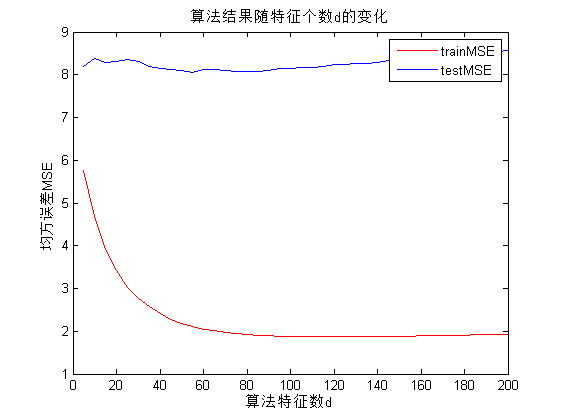
\includegraphics[scale=0.5]{d.png}
    \caption{算法结果随特征个数d的变化}
\end{figure}
\begin{figure}[!htbp]
    \centering
    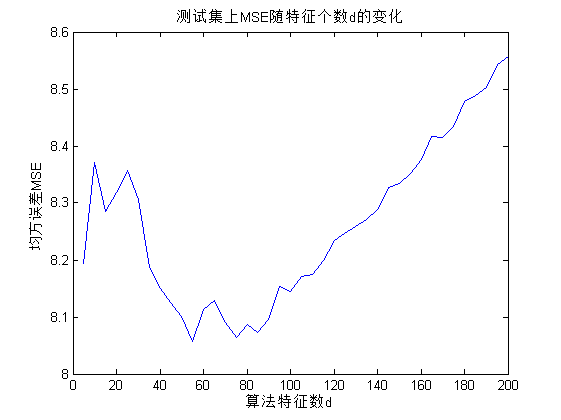
\includegraphics[scale=0.5]{dtest.png}
    \caption{测试集上的MSE随特征个数d的变化}
    \label{d}
\end{figure}

根据图\ref{d},可以看出当d取值在40至60时,在训练数据和测试数据上均体现出较低的MSE。在从算法复杂度的角度考虑,选择d的数值为40。

\subsubsection{超参数$\lambda$}

超参数$\lambda$是控制低秩程度的参数,也具有防止过拟合的作用,不同的$\lambda$会对最终的MSE结果产生直接的影响。改变$\lambda$的数值,其他参数固定(d = 40, Iterations = 5)。$\lambda$的取值分别从0.01取到0.50,间隔为0.01,运行得到的结果如\ref{lambda}所示。

\begin{figure}[!htbp]
    \centering
    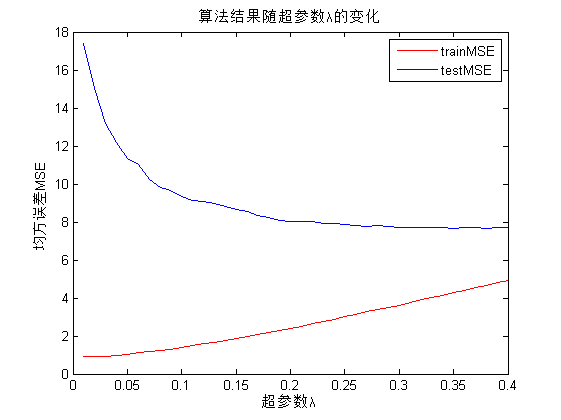
\includegraphics[scale=0.5]{lambda.png}
    \caption{算法结果随超参数$\lambda$的变化}
    \label{lambda}
\end{figure}

根据图\ref{lambda},可以看出当$\lambda$取值在0.40左右时,算法的性能较好。

\subsubsection{迭代次数Iterations}

一般来说,随着迭代次数的增加,MSE会逐渐收敛到最小值。但是迭代次数过多不仅会造成时间复杂度的增加,还有可能导致过拟合现象的发生。因而,选择合适的迭代次数也对算法性能有非常重要的影响。

图\ref{Iter}展示了算法在测试集和训练集上的MSE随着迭代次数增加的变化情况。从图中可以看出迭代次数大概在30至40次时已经收敛,此时迭代次数增加反而可能导致MSE增加。

\begin{figure}[!htbp]
    \centering
    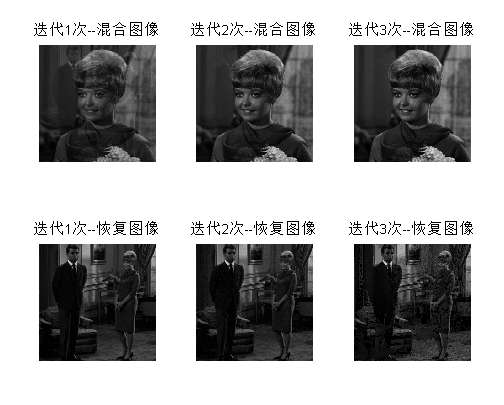
\includegraphics[scale=0.5]{Iter.png}
    \caption{算法结果随迭代次数的变化}
    \label{Iter}
\end{figure}

\subsection{算法收敛时间}
\subsubsection{理论时间复杂度}

假设矩阵\textbf{M}中评分点的个数为$n_r$,由先验可得矩阵\textbf{M}高度稀疏,所以可以得到$n_r << m\times n$。不妨记用户个数为m,电影数目为n,选择的特征个数为d,算法迭代次数为$n_i$。

对于ALS-WR算法,每次更新矩阵\textbf{U}的时间复杂度为$O(d^2(n_r+d\times m))$,每次更新矩阵\textbf{V}的时间复杂度为$O(d^2(n_r + d\times n))$。根据总的迭代次数为$n_i$,则总的时间复杂度为$O(d^2(n_r+d\times(m + n)))$。因此可以得到,当算法使用的特征个数d、迭代次数$n_i$、用户数m、电影数n固定时,时间复杂度主要取决于矩阵\textbf{M}中已有评分数据的个数。

\subsubsection{最终参数选择}

根据上文\textbf{参数的选择}部分的分析,暂时选择的参数为:特征个数d为40左右,超参数$\lambda$为0.40左右,迭代次数Iterations为30左右。选择这些参数的假设是各参数对算法MSE的作用是独立的,实际可能并不满足这一假设。但是通过手动微调,发现这一参数组合性能比较稳定\footnote{由于整体的训练集和测试集是随机选择的,因而算法每次运行的结果不固定,可能会有其他的参数组合在某次运行中得到个别的更小的MSE,但是不够稳定。},MSE结果浮动不大,因而将这一结果作为最终选择的参数。

\subsubsection{算法收敛时间及均方误差}
在选定的参数组合下,最后达到的均方误差为7.80左右浮动(图\ref{MSE}),MATLAB运行时间在38s左右浮动(图\ref{time})。

\begin{figure}[!htbp]
    \centering
    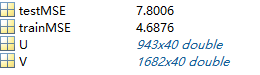
\includegraphics[scale=0.8]{MSE.png}
    \caption{ALS-WR均方误差(最佳)}
    \label{MSE}
\end{figure}
\begin{figure}[!htbp]
    \centering
    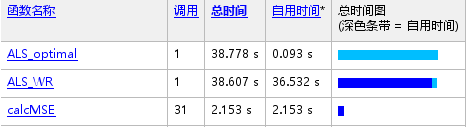
\includegraphics[scale=0.6]{time.png}
    \caption{ALS-WR算法MATLAB运行时间}
    \label{time}
\end{figure}

\section{正则化奇异值分解}
本文重点呈现了最小二乘法在填充矩阵问题中的应用。在推荐系统中,还有一个广泛应用的算法为奇异值分解(Singular Value Decomposition, SVD)算法。本文参考了文献\cite{SVD}和\cite{RSVD},也基于作业提供的数据实现了改进版的SVD算法——正则化奇异值分解(Regularized Singular Value Decomposition, SVD)。因算法实现结果在时间长度和MSE上均不如ALS-WR算法的性能,因而不在文中具体阐述(具体步骤详见代码)。通过与ALS-WR算法类似的算法分析$\rightarrow$算法实现$\rightarrow$ 参数选择等过程,同样可以在测试集上达到8.0左右的均方误差(MSE),略微高于ALS-WR算法的7.80。

\section{总结}
本文主要使用加权正则化交替最小二乘法解决了协同滤波中的填充矩阵问题。同时还尝试实现了正则奇异值分解算法,同样能够解决了协同滤波问题。在文中,笔者对ALS-WR算法超参数的选择、性能评价(测试集上的均方误差)和算法的收敛速度分别进行了细致地分析与讨论,最终确定了参数,得到了性能较优的结果,保存得到填充矩阵。

\newpage
\onecolumn
\section{附录}
\subsection{代码清单}
\subsubsection{ALS-WR算法代码}
\begin{table}[!htbp]
  \centering  
  \begin{tabular}{c|c} 
  \hline\hline
  文件名 & 文件功能\\ \hline
  $ALS\_WR.m$ & ALS-WR算法函数代码 \\
  $ALS\_WR\_Iter.m$ & ALS-WR算法调整版(研究迭代次数) \\ \hline
  $ALS\_d.m$ & 研究特征个数d的影响 \\
  $ALS\_lambda.m$ & 研究超参数$\lambda$的影响\\
  $ALS\_Iteration.m$ & 研究迭代次数的影响\\ \hline
  $ALS\_optimal.m$ & 参数确定后的实现代码 \\
  calcMSE.m & 计算训练数据或测试数据上的均方误差(MSE) \\
  \hline\hline
\end{tabular}
\caption{ALS-WR算法代码清单}
\end{table}

\subsubsection{RSVD算法代码}
\begin{table}[!htbp]
  \centering  
  \begin{tabular}{c|c} 
  \hline\hline
  文件名 & 文件功能\\ \hline
  RSVD.m & RSVD算法实现代码 \\ \hline
  $mean\_calc.m$& 函数:计算训练数据均值 \\
  $bias\_calc.m$ & 函数:计算用户和电影的属性值 \\
  \hline\hline
\end{tabular}
\caption{RSVD算法代码清单}
\end{table}

\subsection{程序运行说明}
本文实现的目前最小MSE为7.80,相应的矩阵\textbf{X}存储在X.mat中。其中,ALS-WR算法请直接运行ALS-WR文件内的ALS\_optimal.m脚本文件,等待约40s即可输出得到结果;RSVD算法请直接运行RSVD文件内的RSVD.m脚本运行,时间稍长,需要约3分钟输出结果。

如果老师/助教在运行中出现任何问题,请联系liuqian14@mails.tsinghua.edu.cn,谢谢!


\begin{thebibliography}{1}
\addcontentsline{toc}{section}{7. 参考文献}
\bibitem{Net}
Zhou Y, Wilkinson D, Schreiber R, et al. Large-Scale Parallel Collaborative Filtering for the Netflix Prize[C]. Algorithmic Aspects in Information and Management, International Conference, Aaim 2008, Shanghai, China, June 23-25, 2008. Proceedings. DBLP, 2008:337-348.

\bibitem{ALSWR}
李改, 李磊等. 基于矩阵分解的协同过滤算法[J]. 计算机工程与应用, 2011, 47(30):4-7.

\bibitem{SVD}
Ma, Chih Chao. A Guide to Singular Value Decomposition for Collaborative Filtering[J]. 2008.

\bibitem{RSVD}
Koren Y. The bellkor solution to the netflix grand prize[J]. Netflix Prize Documentation, 2009.
\end{thebibliography}

\end{document}